\begin{frame}{もろもろ作成}
   \begin{columns}[t]
    \begin{column}{0.6\textwidth}
      <もろもろ作成の概要>
      \begin{itemize}
        \item[(1)]<1-> 1/8ショートケーキモデルの \\
                       各対称面を拘束 
        \item[(2)]<2-> つづいて面圧を設定
      \end{itemize}
    \end{column}
    \begin{column}{0.4\textwidth}
      \vspace{-7mm}
      \begin{figure}[htbp]
        \begin{center}
          \begin{overlayarea}{7cm}{15cm}
            \only<1>{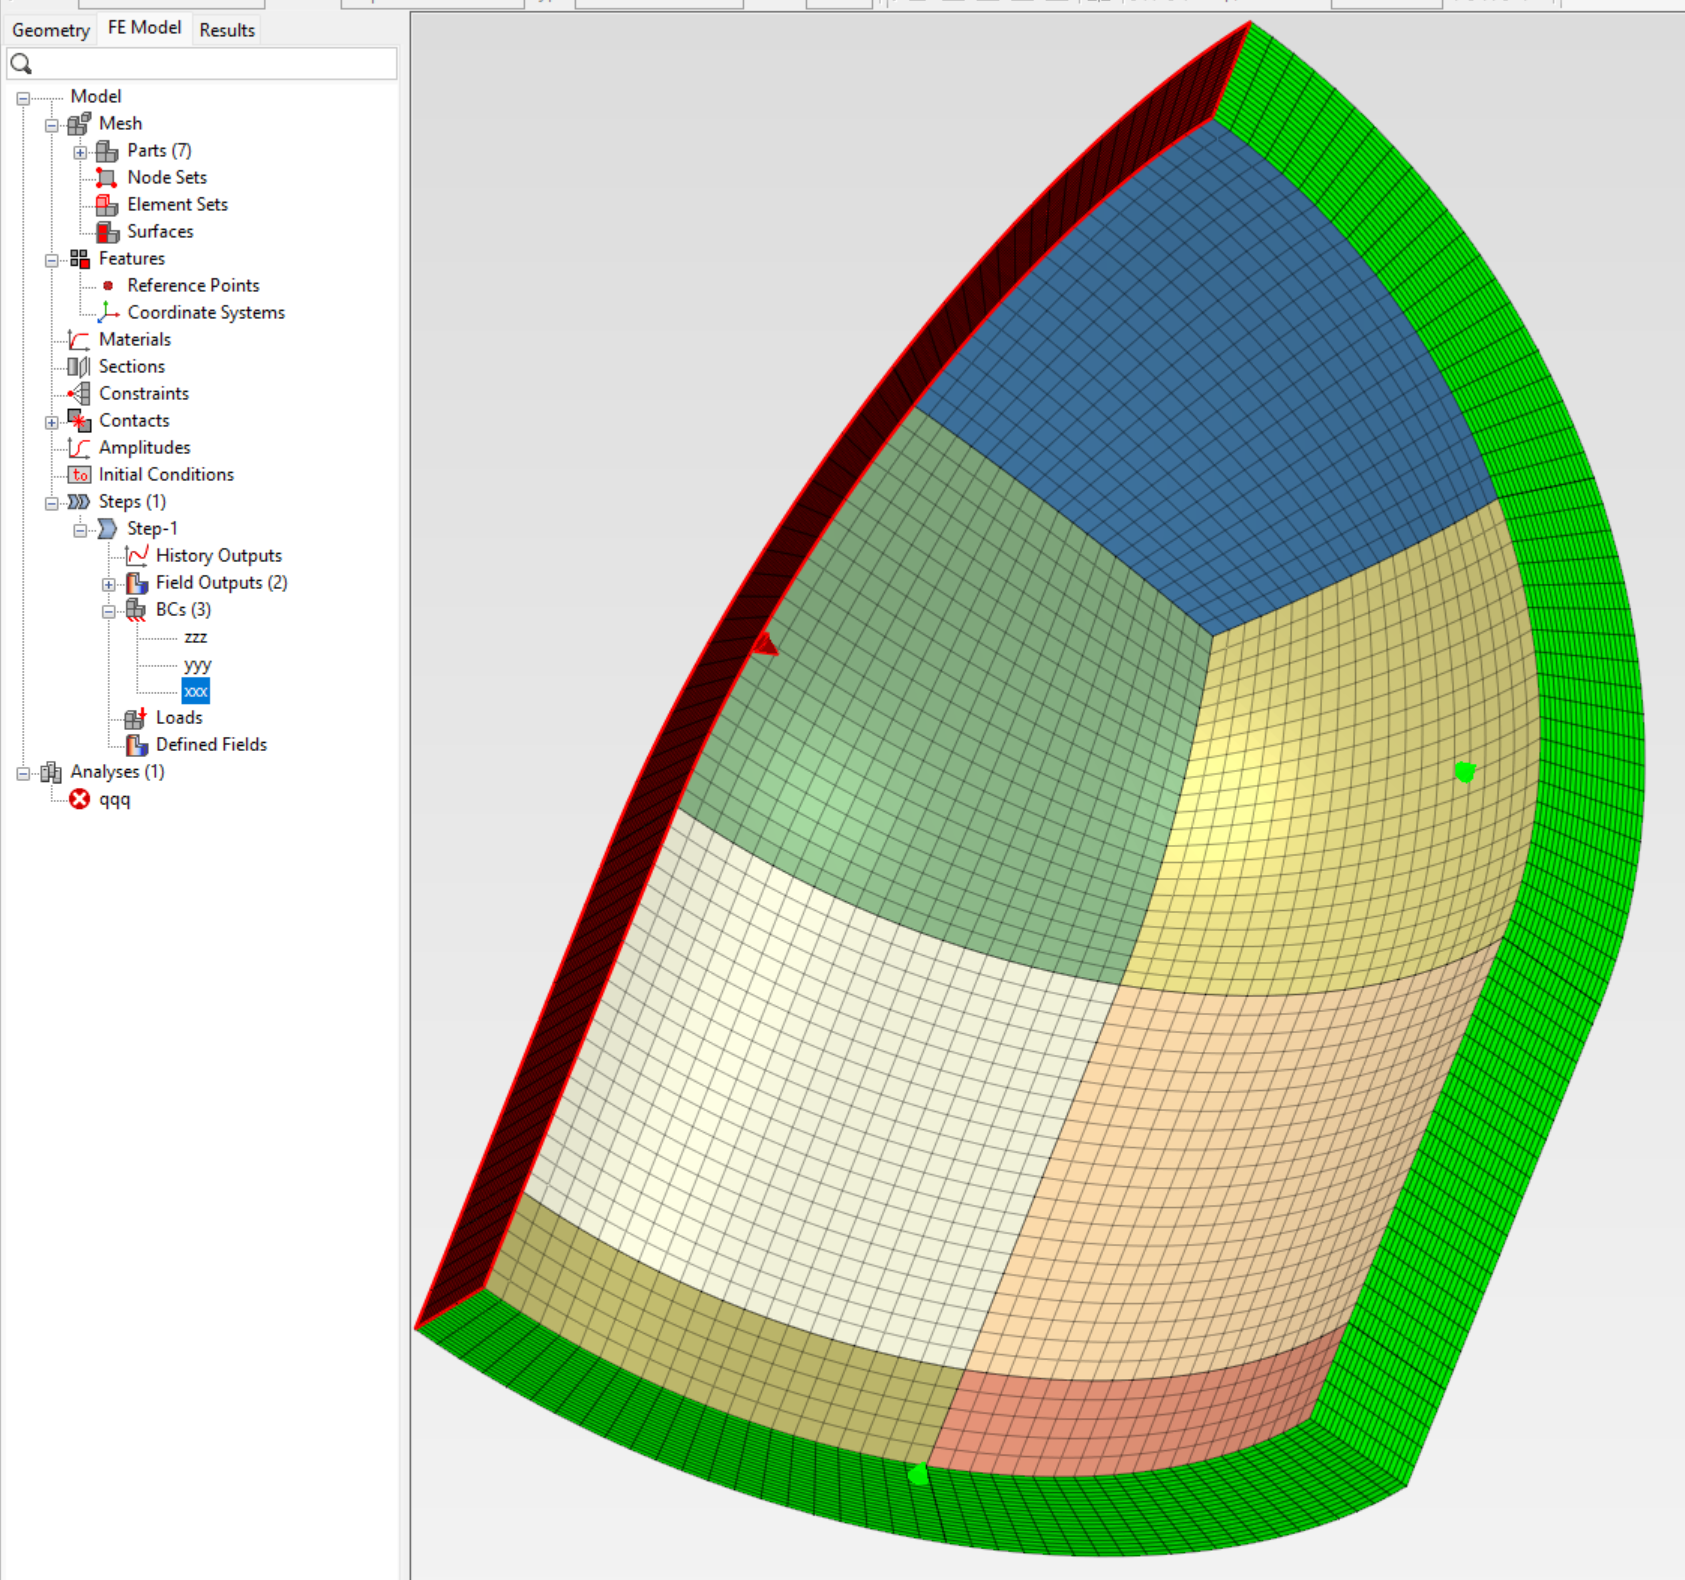
\includegraphics[keepaspectratio,scale=0.30]{images/sc12.png}}
            \only<2>{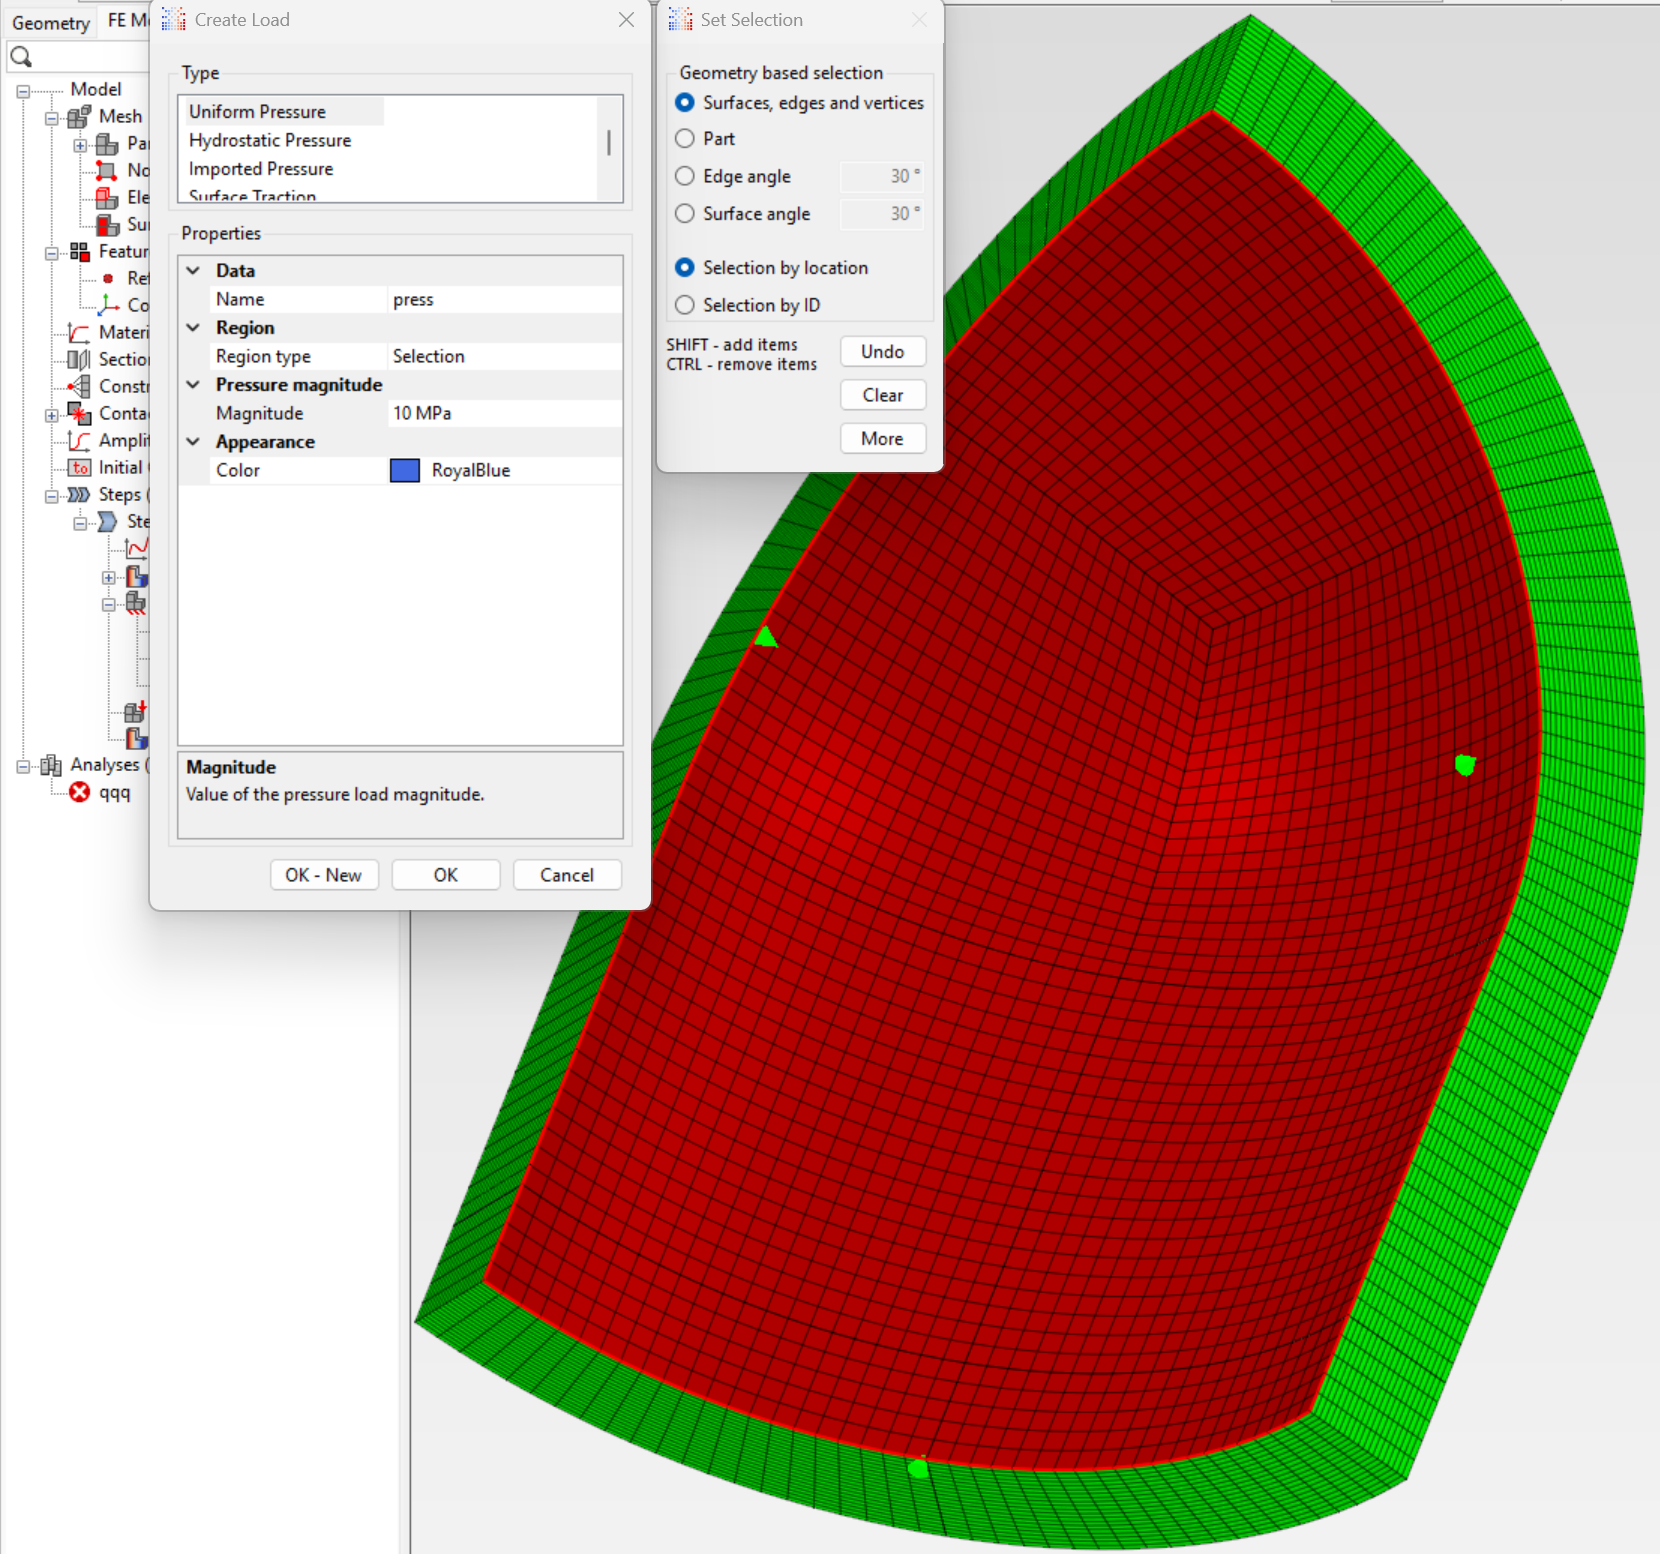
\includegraphics[keepaspectratio,scale=0.30]{images/sc13.png}}
            \caption{もろもろ作成の概要}
          \end{overlayarea}
        \end{center}
      \end{figure}
    \end{column}
  \end{columns}
  \only<1>{
    \begin{textblock*}{160pt}(200pt,73pt)
      \begin{tikzpicture}
         \node[rectangle,fill=cud_yellow,text width=90pt,text centered,rounded corners,minimum height=40pt](s) at (1cm,1cm) { \scriptsize 全体のメッシュ\\サイズを4mmに設定};
         \draw[->, draw=cud_red, line width=1pt] (10pt,50pt) -- (80pt,100pt);
      \end{tikzpicture}
    \end{textblock*}
  }
	  \only<2>{
    \begin{textblock*}{160pt}(195pt,75pt)
      \begin{tikzpicture}
         \node[rectangle,fill=cud_yellow,text width=90pt,text centered,rounded corners,minimum height=40pt](s) at (1cm,1cm) { \scriptsize Second Order\\は No};
         \draw[->, draw=cud_red, line width=1pt] (10pt,50pt) -- (80pt,76pt);
      \end{tikzpicture}
    \end{textblock*}
  }
\end{frame}
